\section{La revue de code}
La revue de code représente une démarche que nous avions mis en avant dans le plan qualité. L'objectif visé est de tendre vers un projet dont l'intégralité du code a été revu. 

La revue de code se fait au moment de l'intégration, c'est pourquoi toutes intégrations nécessitent la création préalable d'une \PullRequest. Pour cela, une fois le travail correspondant à une \UserStory{} est fini\footnote{selon nos critères définis lors de la présentation de la méthode \Scrum{} \ref{methodeScrum}}, le développeur crée une \PullRequest{} via l'outil \Github. Cette \PullRequest s'accompagne d'une description plus technique de la \UserStory{} à laquelle elle est liée. La liste des \Commits{} associés et le code source ajouté et/ou modifié est accessible comme l'on peut le constater ci-dessous. 
\begin{figure}[H]
	\centering
	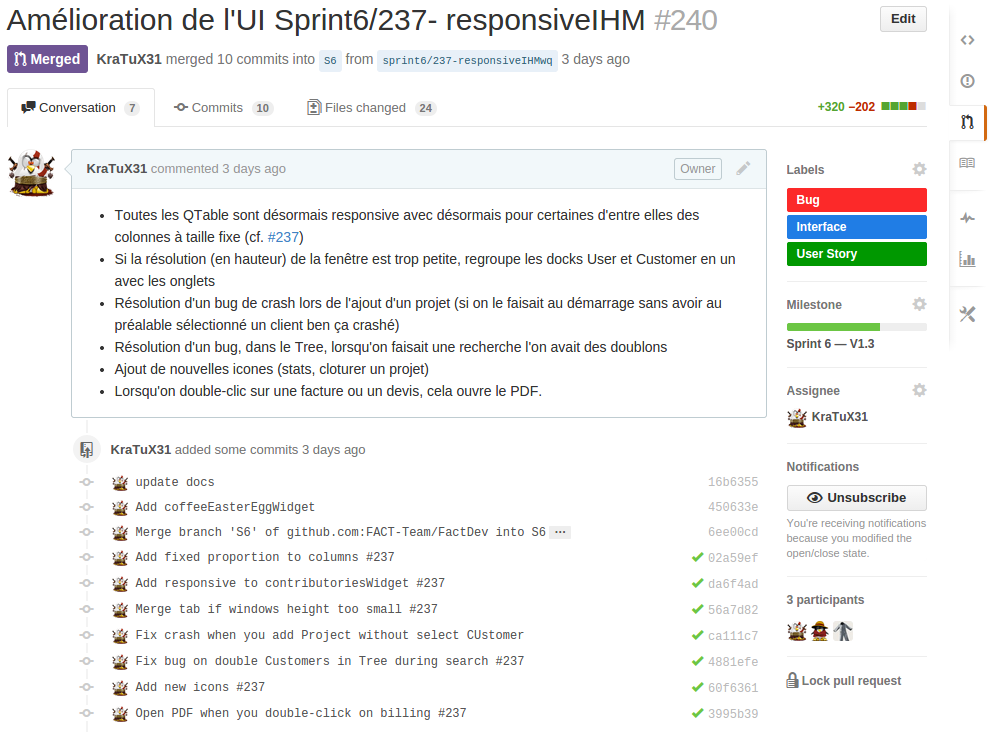
\includegraphics[width=0.7\linewidth]{screens/creation_pr_github}
	\caption{Exemple de \PullRequest{} du projet \FactDev}
	\label{fig:creation_pr_github}
\end{figure}

\`A partir de cette \PullRequest, les autres membres de l'équipe reçoivent une notification pour indiquer qu'ils doivent procéder à la revue de code. Au moins l'un deux doit s'assurer que le code est valide. Un code est dit valide lorsqu'il :
\begin{description}
	\item[est lisible] Le code doit être facile à lire. 
	\item[est compréhensible] Le code doit être facilement compréhensible, avoir un niveau de complexité minimum.
	\item[respecte les conventions d'écritures] Respect des conventions d'écritures (convention de nommage et de mise en forme).
\end{description}

Cette vérification est aisé via l'outil \Github{} qui permet de rajouter des commentaires \textit{« inline »} c'est-à-dire d'ajouter un commentaire aux lignes précise de code à modifier. Ainsi, sans toucher au code, l'on sait précisément l'endroit où l'on doit procéder à des changements. 
\begin{figure}[H]
	\centering
	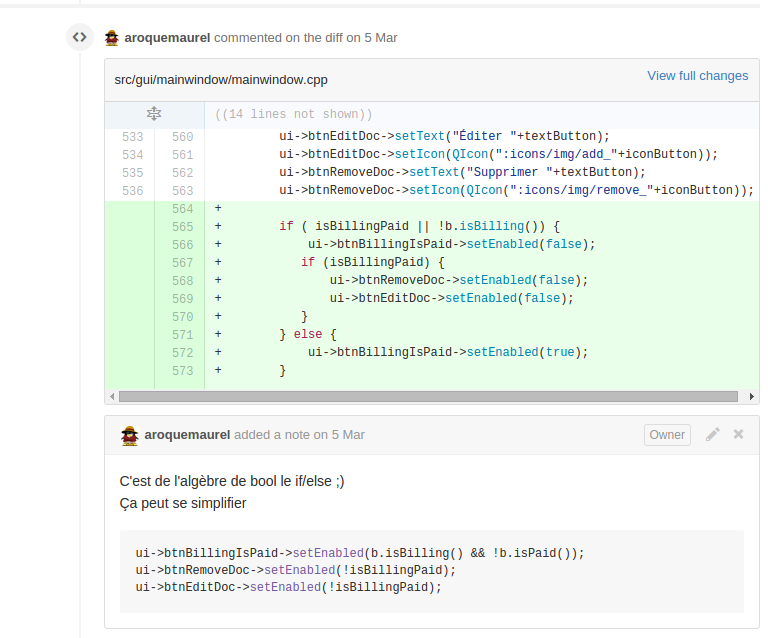
\includegraphics[width=0.7\linewidth]{screens/comments_inline}
	\caption{Ajout d'un commentaire « inline » lors d'une \PullRequest}
	\label{fig:comments_inline}
\end{figure}

L'on procède également à la vérification de la documentation. Chaque méthode et attribut doit être documenté. Là aussi, il faut que la documentation respecte les conventions d'écritures. 

Une fois les remarques faites sur le code et sa documentation, l'on passe aux tests fonctionnels. On se rend donc sur la branche \Git{} en question et l'on vérifie que la fonction répond bien à la \UserStory{} et qu'il n'existe aucun bug. Bien entendu, on s'assure que ça n'a pas entraîné de régression sur d'autres parties du logiciel. C'est aussi le moment de proposer des modifications sur le plan ergonomique si besoin est.  

Enfin, avant d'intégrer, l'on vérifie que les outils (\Travis{} et \Coveralls) ne s'y opposent pas c'est-à-dire que :
\begin{itemize}
	\item le \Build{}\footnote{Un \Build est un artefact logiciel autonome résultant de conversion de fichiers de code source en code exécutable} passe, c'est-à-dire qu'il compile sans erreur.
	\item la couverture de code n'a pas régressé 
\end{itemize}
